% Chapter Template

\chapter{Simulation and Results} % Main chapter title

\label{Chapter4} 
In this chapter, we present the results of our backtesting simulations for different shares, lookback days, breakout percentages, and strategies. We evaluate the performance of each strategy based on the cumulative returns of the portfolio and compare it with the benchmark buy-and-hold strategy. The following tables show the results of the backtesting experiments conducted for the year 2022 with an initial capital of \$100,000.

\section{Backtesting Results for Performance of Different Shares}

\begin{table}[h!]
\centering
\caption{Backtesting Results for Performance of Different Shares}
\label{table:backtesting1}
\begin{tabular}{|c|c|c|c|c|}
\hline
\textbf{Share} & \textbf{Strategy} & \textbf{Lookback Days} & \textbf{Breakout \%} & \textbf{Total Return \%} \\

Google & Williams\%R & 14 & 20 & 0.022 \\

Apple & Williams\%R & 14 & 20 & 0.003 \\

Microsoft & Williams\%R & 14 & 20 & 0.002 \\

Bitcoin & Williams\%R & 14 & 20 & -114.88 \\

Google & Williams\%R+SMALMA & 14 & 20 & 0.038 \\

Apple & Williams\%R+SMALMA & 14 & 20 & 0.011 \\

Microsoft & Williams\%R+SMALMA & 14 & 20 & 0.024 \\

Bitcoin & Williams\%R+SMALMA & 14 & 20 & 22.294 \\
\hline
\end{tabular}
\end{table}

The backtesting results for the performance of different shares using Williams\%R and Williams\%R+SMALMA strategies with a 14-day lookback period and 20\% breakout percentage show that all shares except Bitcoin yielded positive returns. The addition of SMALMA to the Williams\%R strategy resulted in higher returns for all shares. However, Bitcoin showed a significant positive return with the added SMALMA.


\section{Backtesting Results for Performance of Different Lookback Days}

\begin{table}[h!]
\centering
\caption{Backtesting Results for Performance of Different Lookback Days}
\label{table:backtesting2}
\begin{tabular}{|c|c|c|c|c|c|}
\hline
\textbf{Share} & \textbf{Strategy} & \textbf{Lookback Days} & \textbf{Breakout \%} & \textbf{Total Return \%} \\


Bitcoin & Williams\%R & 14 & 20 & -114.888 \\

Bitcoin & Williams\%R & 20 & 20 & -99.234 \\

Bitcoin & Williams\%R & 26 & 20 & -141.393 \\

Bitcoin & Williams\%R & 32 & 20 & -73.985 \\

Bitcoin & Williams\%R+SMALMA & 14 & 20 & 22.294 \\

Bitcoin & Williams\%R+SMALMA & 20 & 20 & -112.182 \\

Bitcoin & Williams\%R+SMALMA & 26 & 20 & -179.004 \\

Bitcoin & Williams\%R+SMALMA & 32 & 20 & -70.200 \\

\hline
\end{tabular}
\end{table}
The backtesting results for different lookback days on Bitcoin using the Williams\%R strategy and Williams\%R+SMALMA strategy indicate that the performance of the trading strategy is highly dependent on the lookback period. The results suggest that a shorter lookback period of 14 days combined with the Williams\%R+SMALMA strategy generated a positive return of 22.294\%, while longer lookback periods of 20, 26, and 32 days resulted in negative returns ranging from -70.200\% to -179.004\%. These findings suggest that traders need to carefully consider the appropriate lookback period when implementing trading strategies, especially when dealing with highly volatile assets like Bitcoin.
\section{Backtesting Results for Performance of Different Strategies}

\begin{table}[htp]
\centering
\caption{Backtesting Results for Performance of Different Strategies}
\label{table:backtesting4}
\begin{tabular}{|c|c|c|c|c|c|}
\hline
\textbf{Share} & \textbf{Strategy} & \textbf{Lookback Days} & \textbf{Breakout \%} & \textbf{Total Return \%} \\


Google & Williams\%R & 14 & 20 & 0.022 \\


Google & Williams\%R+SMALMA & 14 & 20 & 0.039 \\

Google & VolatilityBreakOut & 14 & 20 & 0 \\

Microsoft & Williams\%R & 14 & 20 & 0.015 \\


Microsoft & Williams\%R+SMALMA & 14 & 20 & 0.024 \\

Microsoft & VolatilityBreakOut & 14 & 20 & 0 \\

Apple & Williams\%R & 14 & 20 & -0.025 \\


Apple & Williams\%R+SMALMA & 14 & 20 & 0.012 \\

Apple & VolatilityBreakOut & 14 & 20 & 0 \\

Bitcoin & Williams\%R & 14 & 20 & -114.888 \\


Bitcoin & Williams\%R+SMALMA & 14 & 20 & 22.294 \\

Bitcoin & VolatilityBreakOut & 14 & 20 & 4.8 \\


\hline
\end{tabular}
\end{table}

The backtesting results for different strategies on multiple shares show that Williams\%R+SMALMA is the most profitable strategy for Google, Microsoft, and Apple, whereas VolatilityBreakOut is the most profitable strategy for Bitcoin. However, Williams\%R and VolatilityBreakOut strategies did not show any significant positive returns for any of the shares.
\section{Backtesting Results for Performance of Different Breakout Percentages}

\begin{table}[h!]
\centering
\caption{Backtesting Results for Performance of Different Breakout Percentages}
\label{table:backtesting4}
\begin{tabular}{|c|c|c|c|c|c|}
\hline
\textbf{Share} & \textbf{Strategy} & \textbf{Lookback Days} & \textbf{Breakout \%} & \textbf{Total Return \%} \\

Google & Williams\%R & 14 & 15 & 0.037 \\
Google & Williams\%R & 14 & 20 & 0.022 \\

Google & Williams\%R & 14 & 25 & 0.022 \\

Google & Williams\%R+SMALMA & 14 & 15 & 0.072 \\
Google & Williams\%R+SMALMA & 14 & 20 & 0.039 \\

Google & Williams\%R+SMALMA & 14 & 25 & 0.002 \\

Apple & Williams\%R & 14 & 15 & 0 \\
Apple & Williams\%R & 14 & 20 & 0 \\

Apple & Williams\%R & 14 & 25 & -0.006 \\

Apple & Williams\%R+SMALMA & 14 & 15 & 0.063 \\
Apple & Williams\%R+SMALMA & 14 & 20 & 0.011 \\

Apple & Williams\%R+SMALMA & 14 & 25 & -0.063 \\



Microsoft & Williams\%R+SMALMA & 14 & 15 & -0.061 \\
Microsoft & Williams\%R+SMALMA & 14 & 20 & -0.024 \\

Microsoft & Williams\%R+SMALMA & 14 & 25 & -0.144 \\

Bitcoin & Williams\%R & 14 & 15 & -117.991 \\
Bitcoin & Williams\%R & 14 & 20 & -114.888 \\

Bitcoin & Williams\%R & 14 & 25 & -145.049 \\

Bitcoin & Williams\%R+SMALMA & 14 & 15 & 239.064 \\
Bitcoin & Williams\%R+SMALMA & 14 & 20 & 22.294 \\

Bitcoin & Williams\%R+SMALMA & 14 & 25 & 71.246 \\





\hline
\end{tabular}
\end{table}

The backtesting results for different breakout percentages show that the performance of the strategies varies significantly with different breakout levels. The Williams\%R+SMALMA strategy performs well with a breakout percentage of 15\% for Google and Apple, but not for Microsoft. The Williams\%R strategy performs better with a breakout percentage of 15\% for Google, but not for Apple or Microsoft. For Bitcoin, the Williams\%R+SMALMA strategy performs significantly better with a breakout percentage of 15\%. 

The table shows the results of backtesting different breakout percentages for four different shares using two different trading strategies. The results indicate that the performance of each strategy and share combination can be highly sensitive to the breakout percentage used. In some cases, small changes in the breakout percentage can result in significantly different returns. These results highlight the importance of selecting the appropriate breakout percentage when implementing a breakout trading strategy. 
% \section{Backtesting Results for Different Shares and Lookback Days}

% \begin{table}[h!]
% \centering
% \caption{Backtesting Results for Different Shares and Lookback Days}
% \label{table:backtesting5}
% \begin{tabular}{|c|c|c|c|c|c|}
% \hline
% \textbf{Share} & \textbf{Strategy} & \textbf{Lookback Days} & \textbf{Breakout \%} & \textbf{Total Return \%} \\


% Google & Williams\%R & 14 & 20 & 20 \\


% Google & Williams\%R+SMALMA & 14 & 20 & 20 \\

% Google & VolatilityBreakOut & 14 & 20 & 20 \\

% Microsoft & Williams\%R & 14 & 20 & 20 \\


% Microsoft & Williams\%R+SMALMA & 14 & 20 & 20 \\

% Microsoft & VolatilityBreakOut & 14 & 20 & 20 \\

% Apple & Williams\%R & 14 & 20 & 20 \\


% Apple & Williams\%R+SMALMA & 14 & 20 & 20 \\

% Apple & VolatilityBreakOut & 14 & 20 & 20 \\

% Bitcoin & Williams\%R & 14 & 20 & 20 \\


% Bitcoin & Williams\%R+SMALMA & 14 & 20 & 20 \\

% Bitcoin & VolatilityBreakOut & 14 & 20 & 20 \\


% \hline
% \textbf{Share} & \textbf{Strategy} & \textbf{Lookback Days} & \textbf{Breakout Percentage} & \textbf{Total Return Percentage}
% \end{tabular}
% \end{table}

% \section{Backtesting Results for Different Shares and Strategies}

% \begin{table}[h!]
% \centering
% \caption{Backtesting Results for Different Shares and Strategies}
% \label{table:backtesting7}
% \begin{tabular}{|c|c|c|c|c|c|}
% \hline
% \textbf{Share} & \textbf{Strategy} & \textbf{Lookback Days} & \textbf{Breakout Percentage} & \textbf{Total Return Percentage}
% \end{tabular}
% \end{table}

\section{Backtesting Results for GOOGL}
Figures show the entry and exit points for Google with a lookback period of 14 days using the different strategy. The green arrows represent the entry points, and the red arrows represent the exit points. The blue line shows the cumulative returns of the portfolio.

The backtesting results for Google in 2022 using the Williams\%R+SMALMA strategy with a lookback of 14 days and a breakout percentage of 20\% showed a positive total return of 3.8\%, which suggests that this strategy was successful in generating profits for Google during this period.

\begin{figure}[h!]
\centering
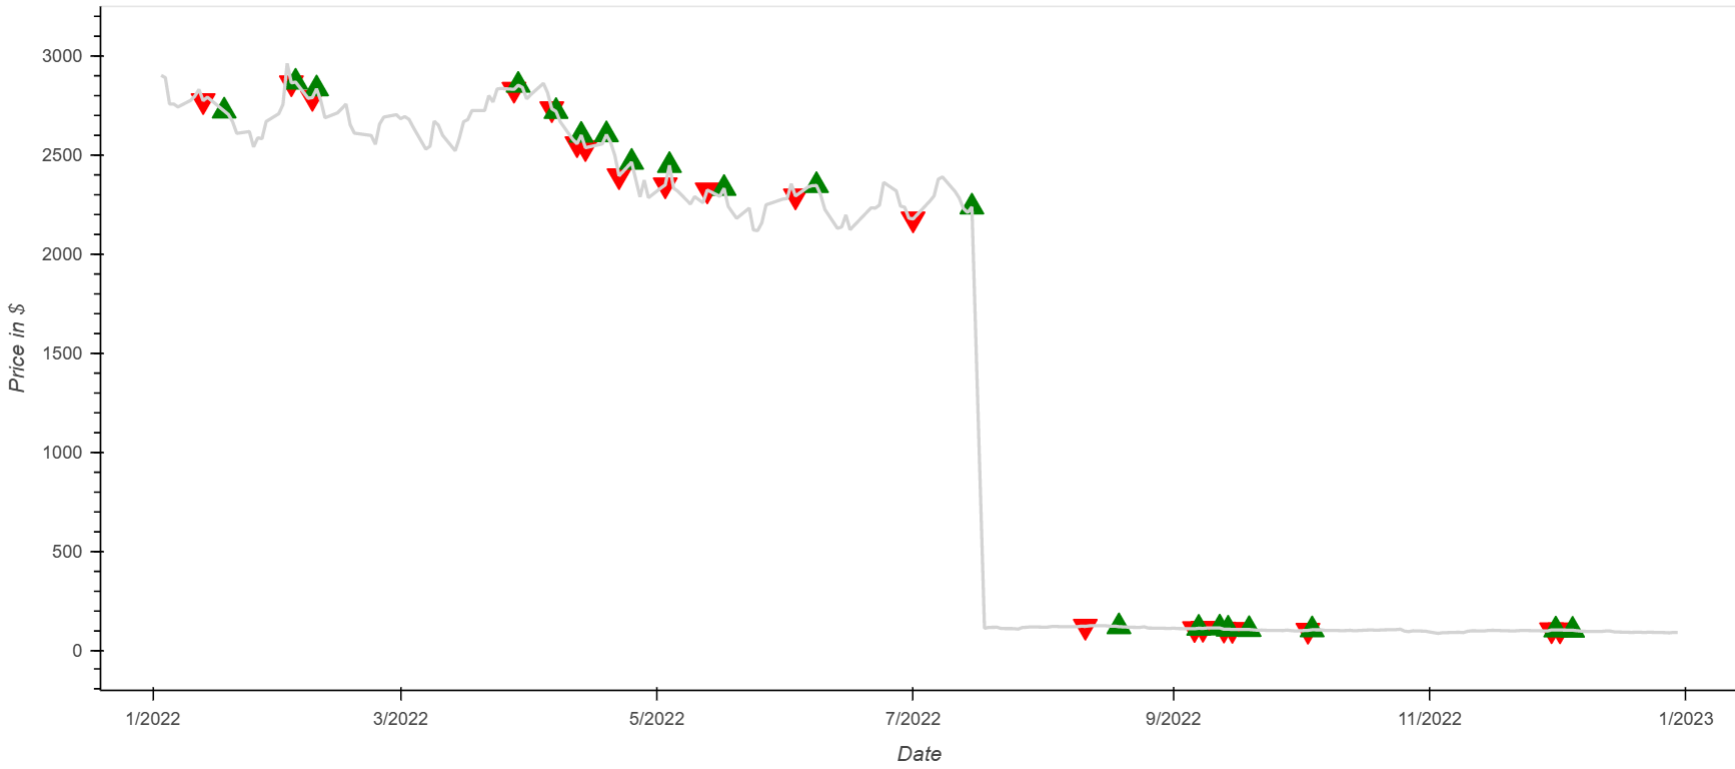
\includegraphics[width=0.8\textwidth]{Images/google_williams_R_1.png}
\caption{Entry and Exit Points for GOOGL (Lookback Period = 14 Days, Breakout Percent = 20, Williams \% R Strategy, Year = 2022)}
\label{fig:entryexit1}
\end{figure}

\begin{figure}[h!]
\centering
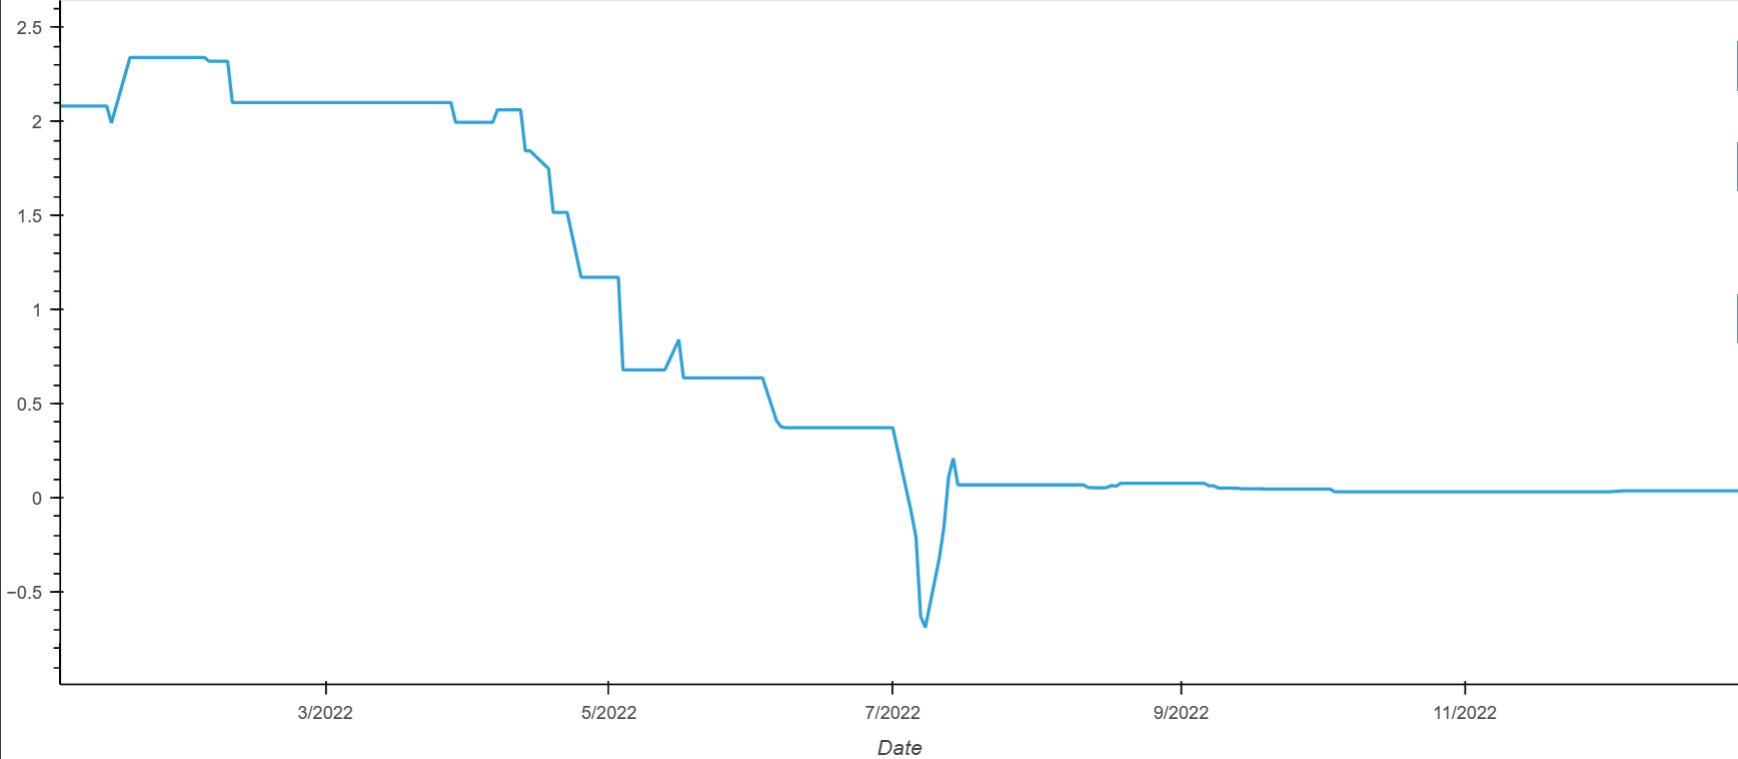
\includegraphics[width=0.8\textwidth]{Images/google_williams_R_2.png}
\caption{Cumulative Returns for GOOGL (Lookback Period = 14 Days, Breakout Percent = 20, Williams \% R Strategy, Year = 2022)}
\label{fig:entryexit1}
\end{figure}

\begin{figure}[h!]
\centering
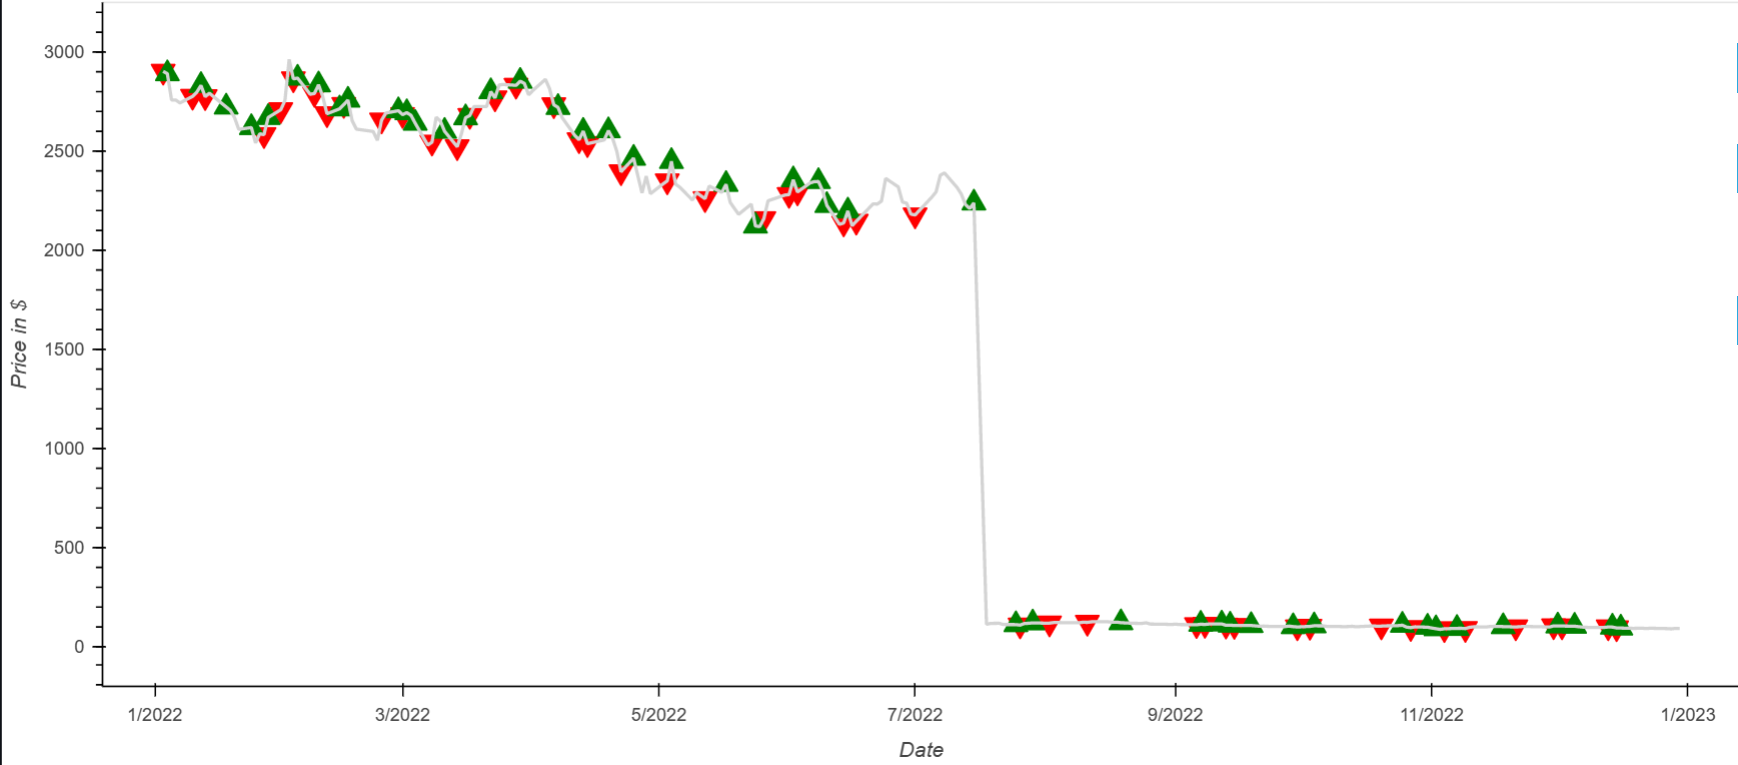
\includegraphics[width=0.8\textwidth]{Images/google_williams_lma__1.png}
\caption{Entry and Exit Points for GOOGL (Lookback Period = 14 Days, Breakout Percent = 20, Williams \% R + LMASMA Strategy, Year = 2022)}
\label{fig:entryexit1}
\end{figure}

\begin{figure}[h!]
\centering
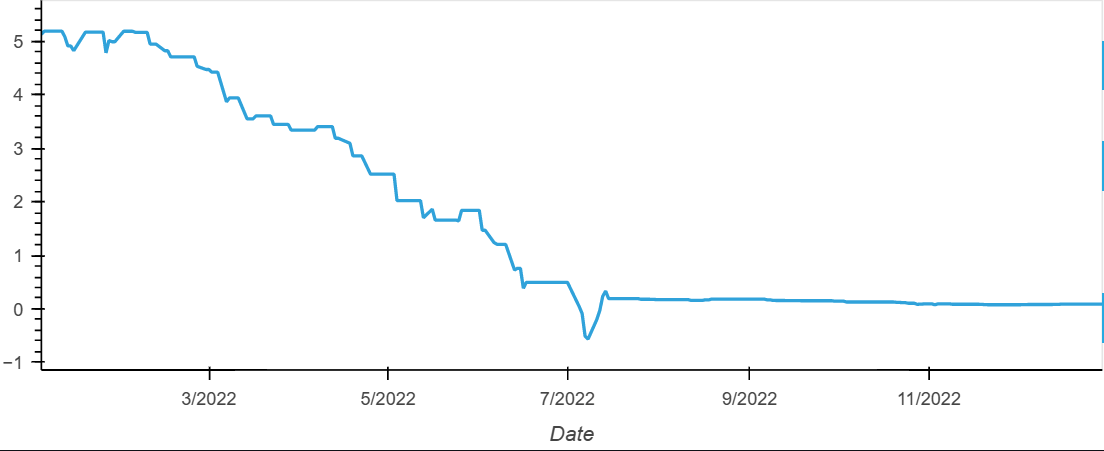
\includegraphics[width=0.8\textwidth]{Images/google_williams_lma__2.png}
\caption{Cumulative for GOOGL (Lookback Period = 14 Days, Breakout Percent = 20, Williams \% R + LMASMA Strategy, Year = 2022)}
\label{fig:entryexit1}
\end{figure}

\begin{figure}[h!]
\centering
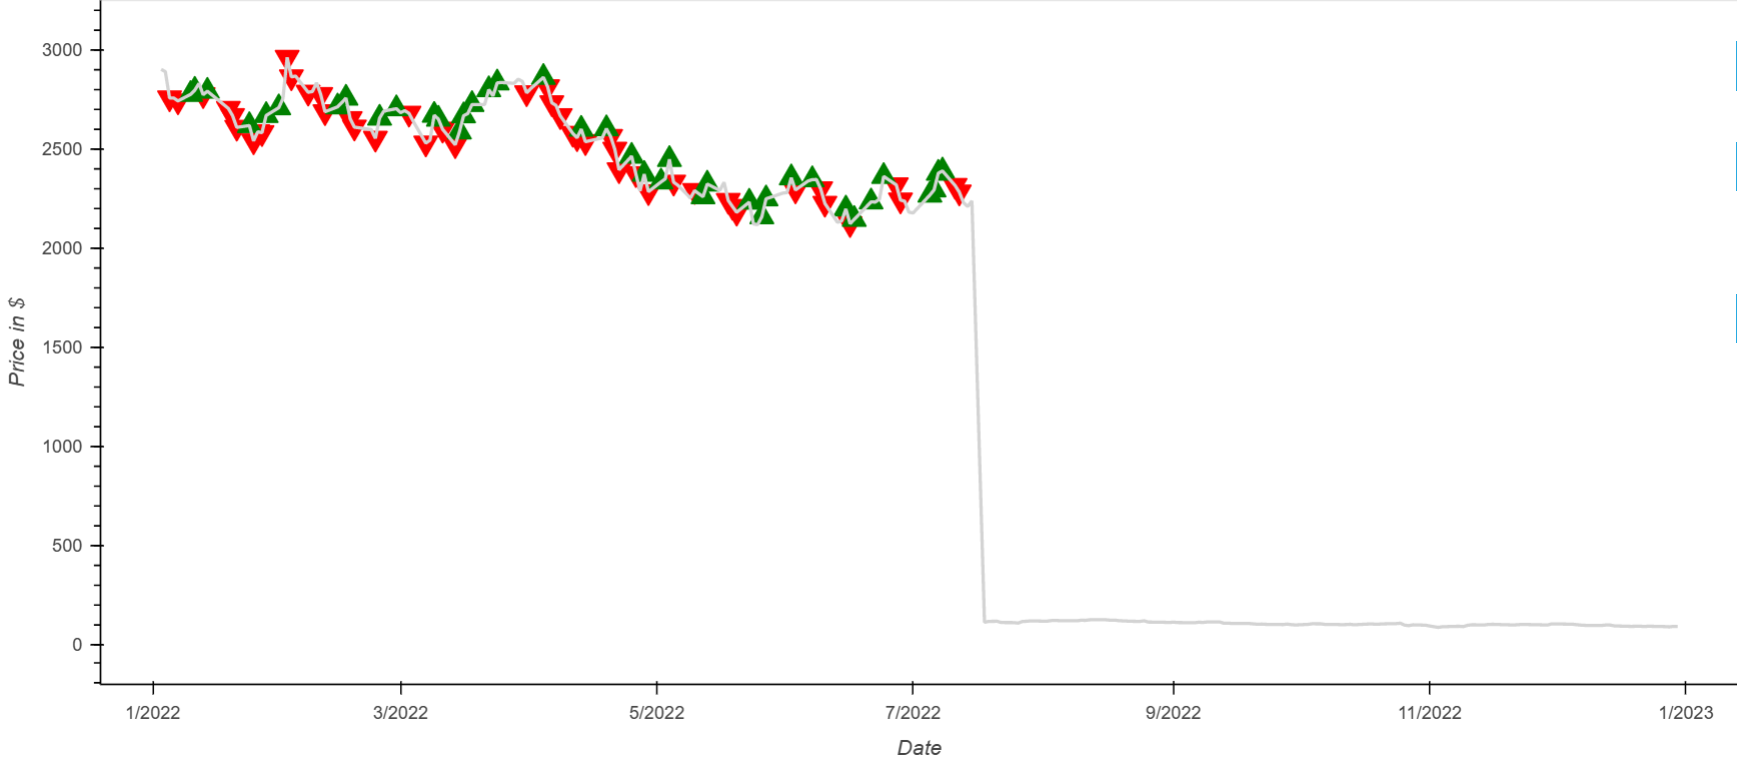
\includegraphics[width=0.8\textwidth]{Images/google_volaitity_1.png}
\caption{Entry and Exit Points for GOOGL (Lookback Period = 14 Days, Breakout Percent = 20, Volatility Breakout Strategy, Year = 2022)}
\label{fig:entryexit1}
\end{figure}

\begin{figure}[h!]
\centering
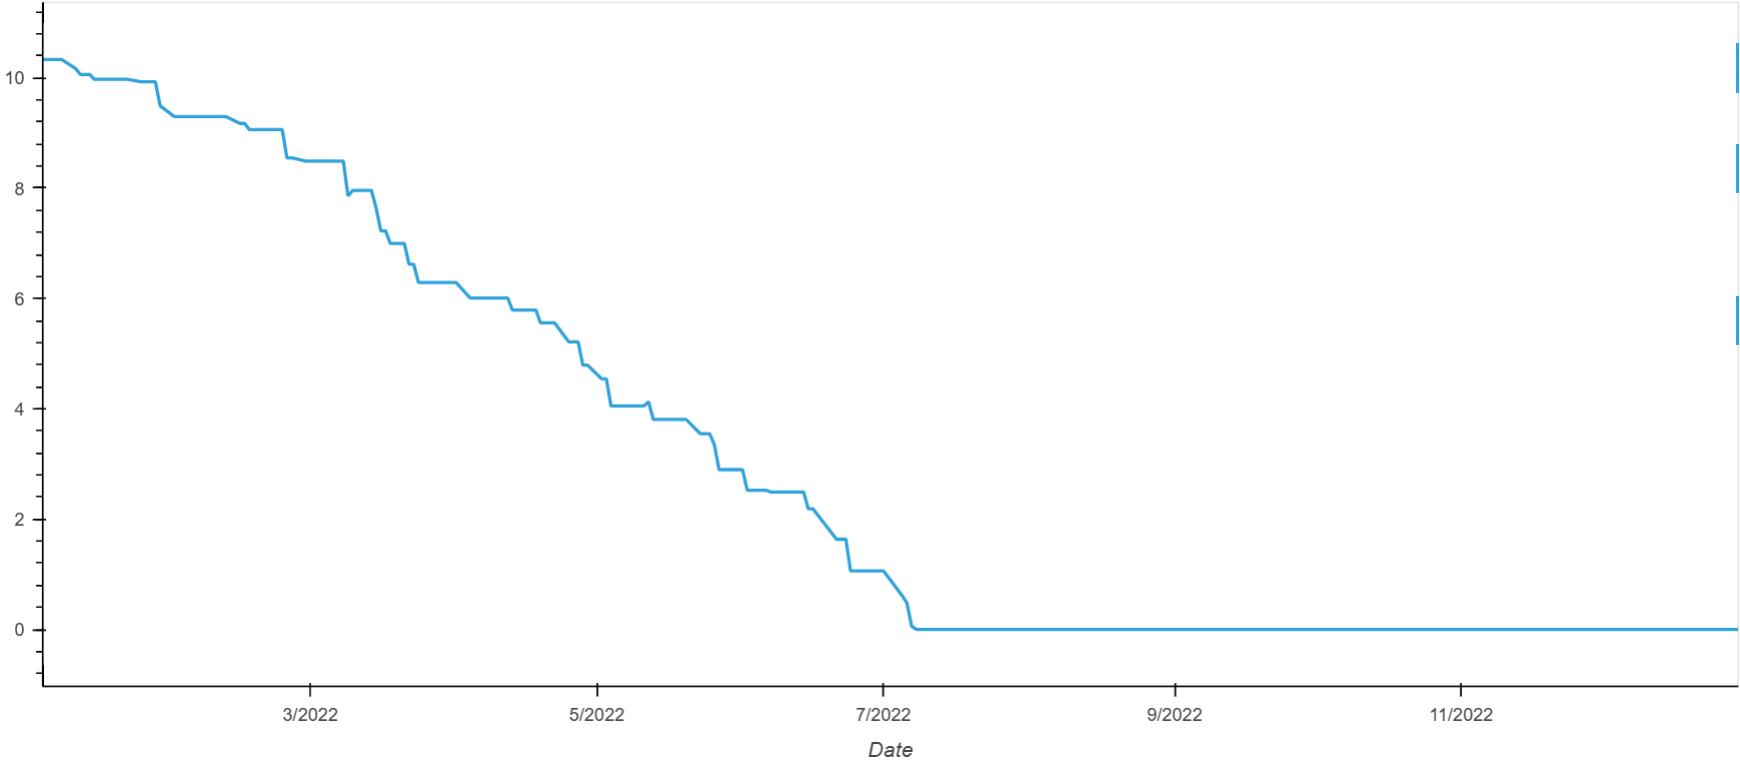
\includegraphics[width=0.8\textwidth]{Images/google_volaitity_2.png}
\caption{Cumulative Returns for GOOGL (Lookback Period = 14 Days, Breakout Percent = 20, Volatility Breakout Strategy, Year = 2022)}
\label{fig:entryexit1}
\end{figure}

\section{Backtesting Results for AAPL}
Figures show the entry and exit points for Apple with a lookback period of 14 days using the different strategy. The green arrows represent the entry points, and the red arrows represent the exit points. The blue line shows the cumulative returns of the portfolio.

The backtesting results of Apple for the year 2022 using Williams\%R+SMALMA strategy showed a positive total return of 0.012\% with a breakout percentage of 20 and a lookback period of 14 days, indicating that this strategy could potentially generate profits for short-term investors in Apple's stock market.

\begin{figure}[h!]
\centering
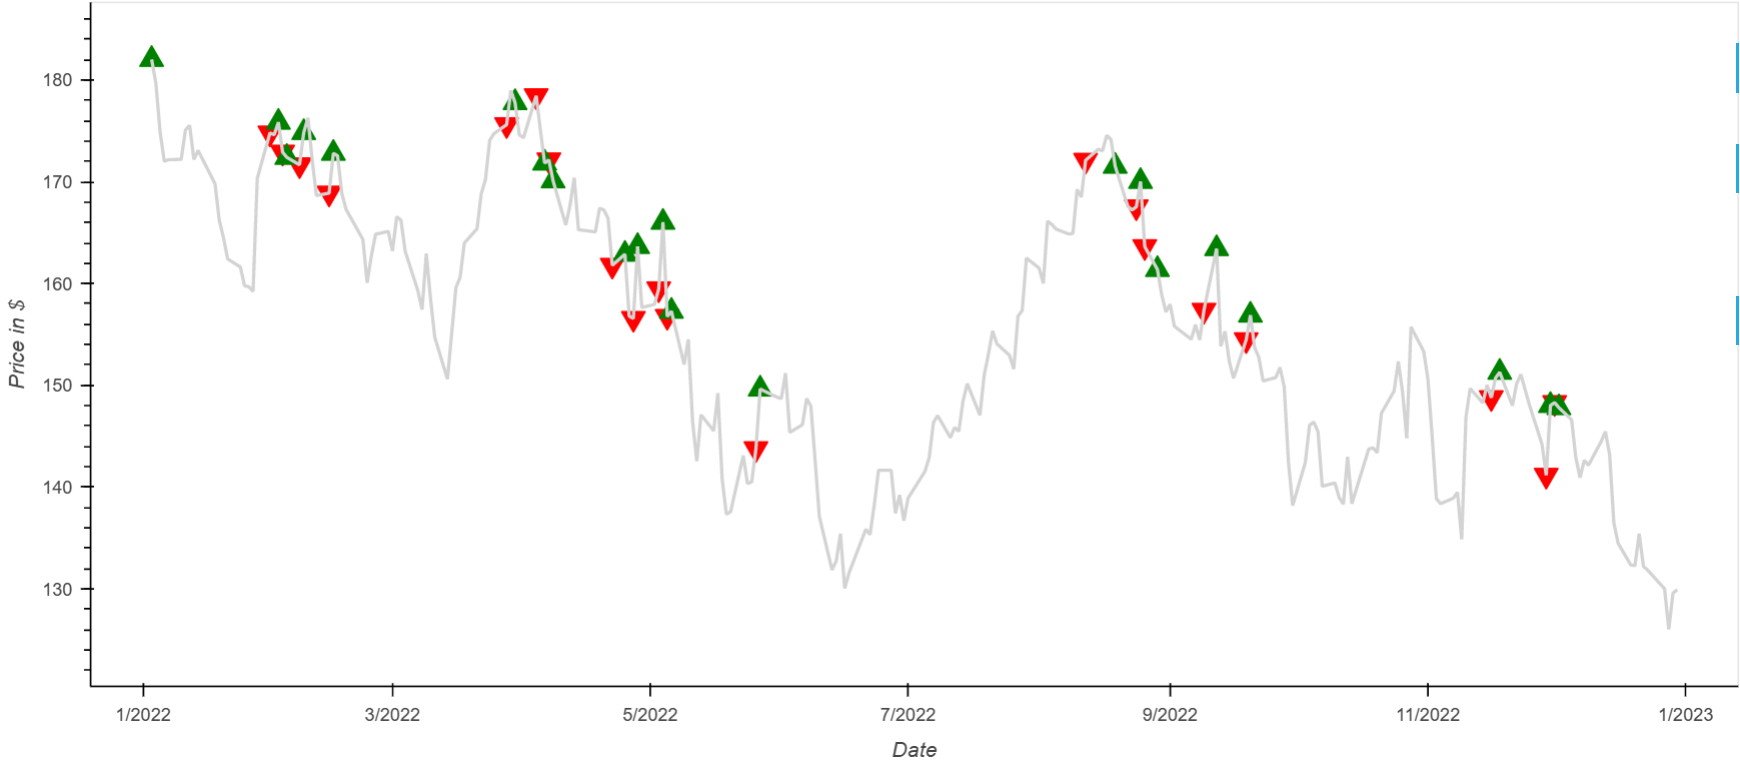
\includegraphics[width=0.8\textwidth]{Images/apple_williams_R_1.png}
\caption{Entry and Exit Points for AAPL (Lookback Period = 14 Days, Breakout Percent = 20, Williams \% R Strategy, Year = 2022)}
\label{fig:entryexit1}
\end{figure}

\begin{figure}[h!]
\centering
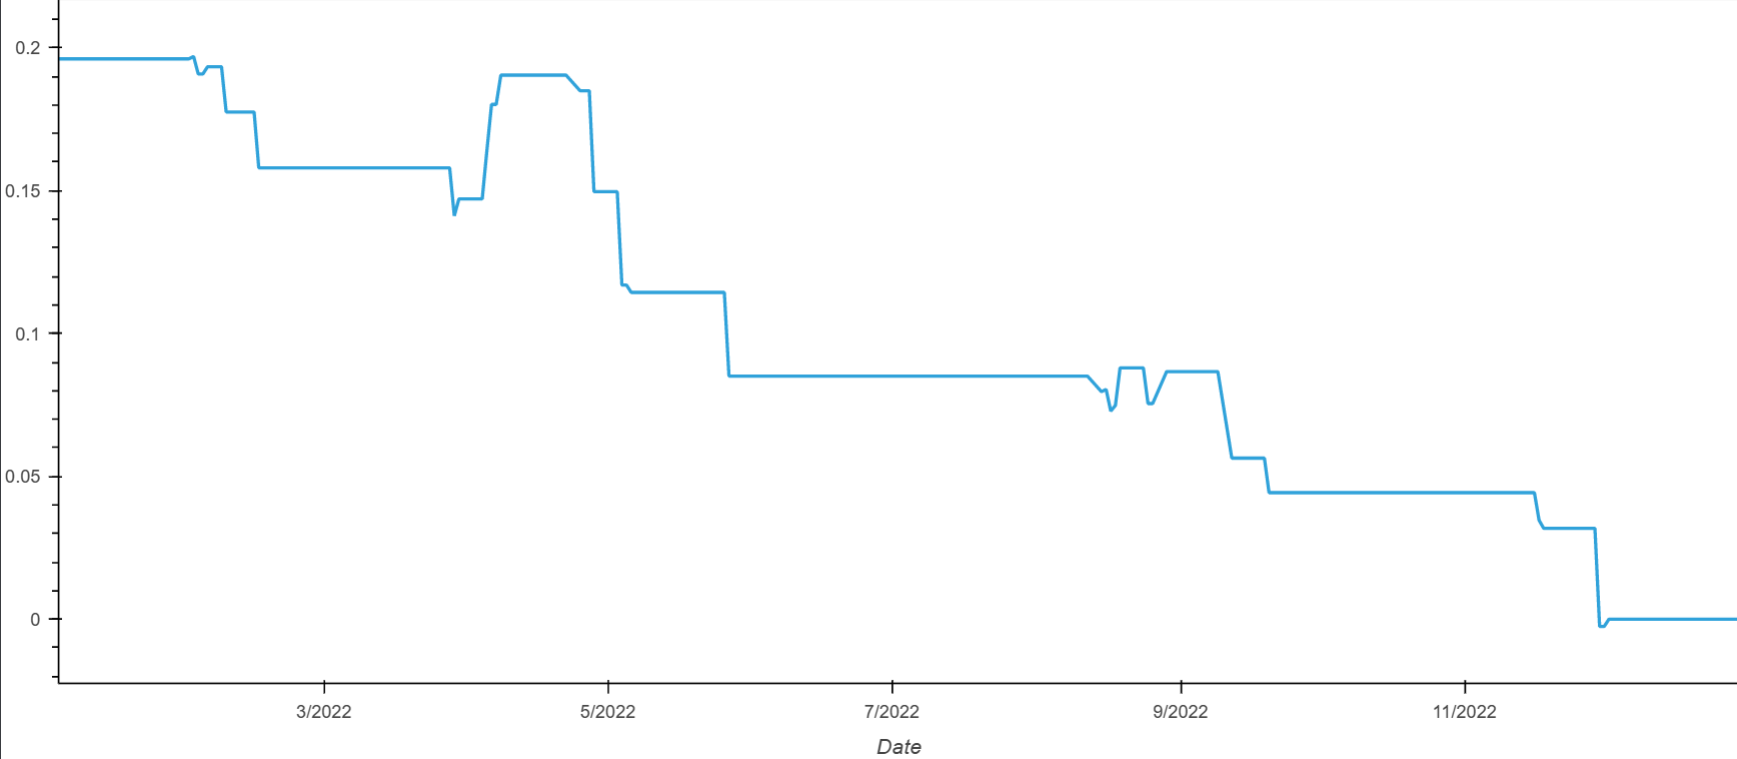
\includegraphics[width=0.8\textwidth]{Images/apple_williams_R_2.png}
\caption{Cumulative Returns for AAPL (Lookback Period = 14 Days, Breakout Percent = 20, Williams \% R Strategy, Year = 2022)}
\label{fig:entryexit1}
\end{figure}

\begin{figure}[h!]
\centering
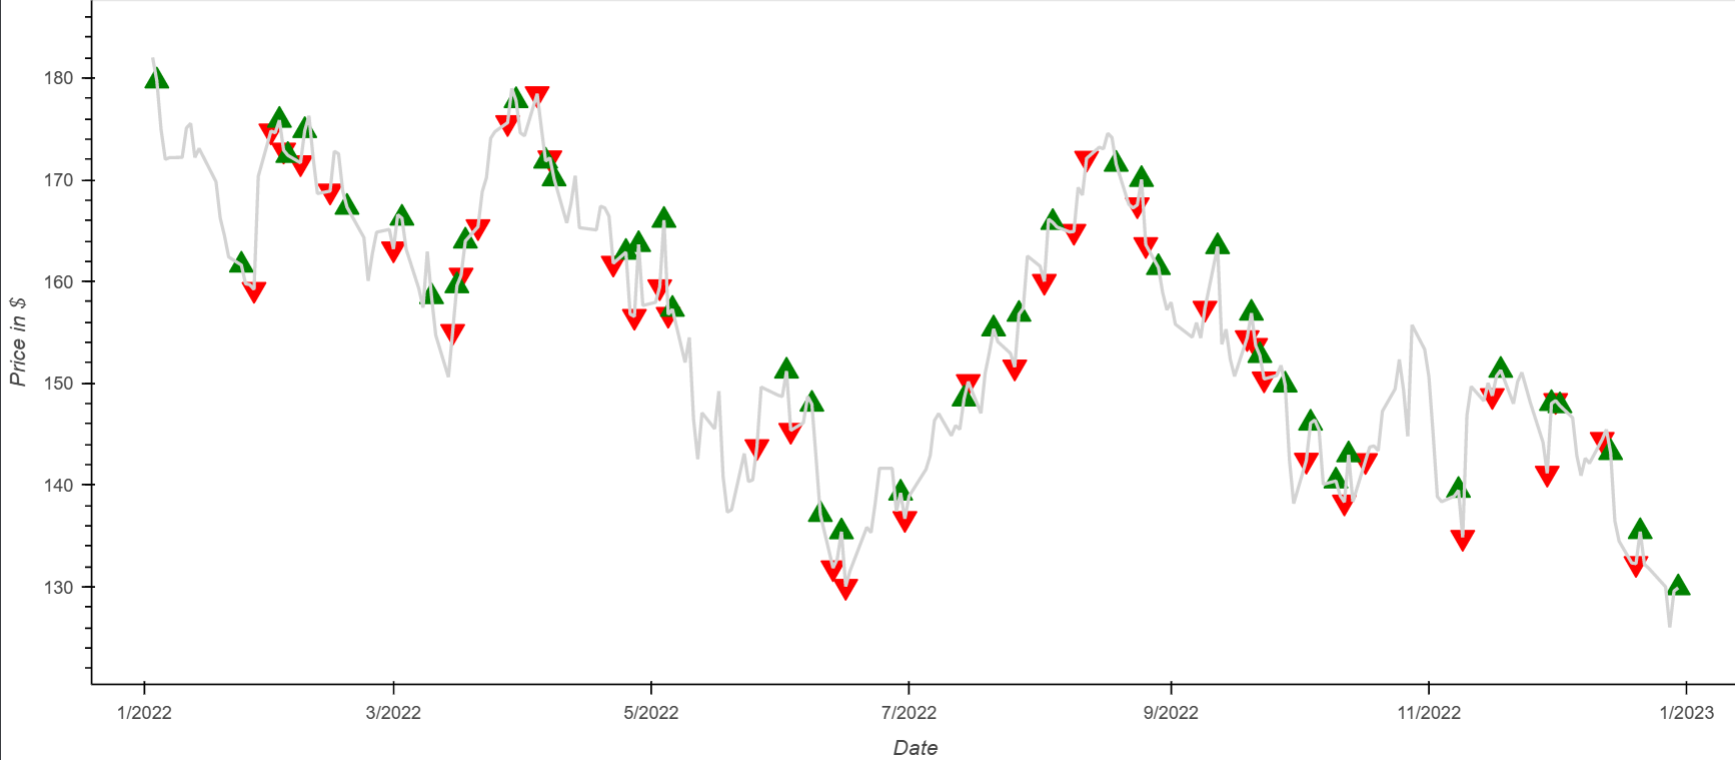
\includegraphics[width=0.8\textwidth]{Images/apple_williams_lma__1.png}
\caption{Entry and Exit Points for AAPL (Lookback Period = 14 Days, Breakout Percent = 20, Williams \% R + LMASMA Strategy, Year = 2022)}
\label{fig:entryexit1}
\end{figure}

\begin{figure}[h!]
\centering
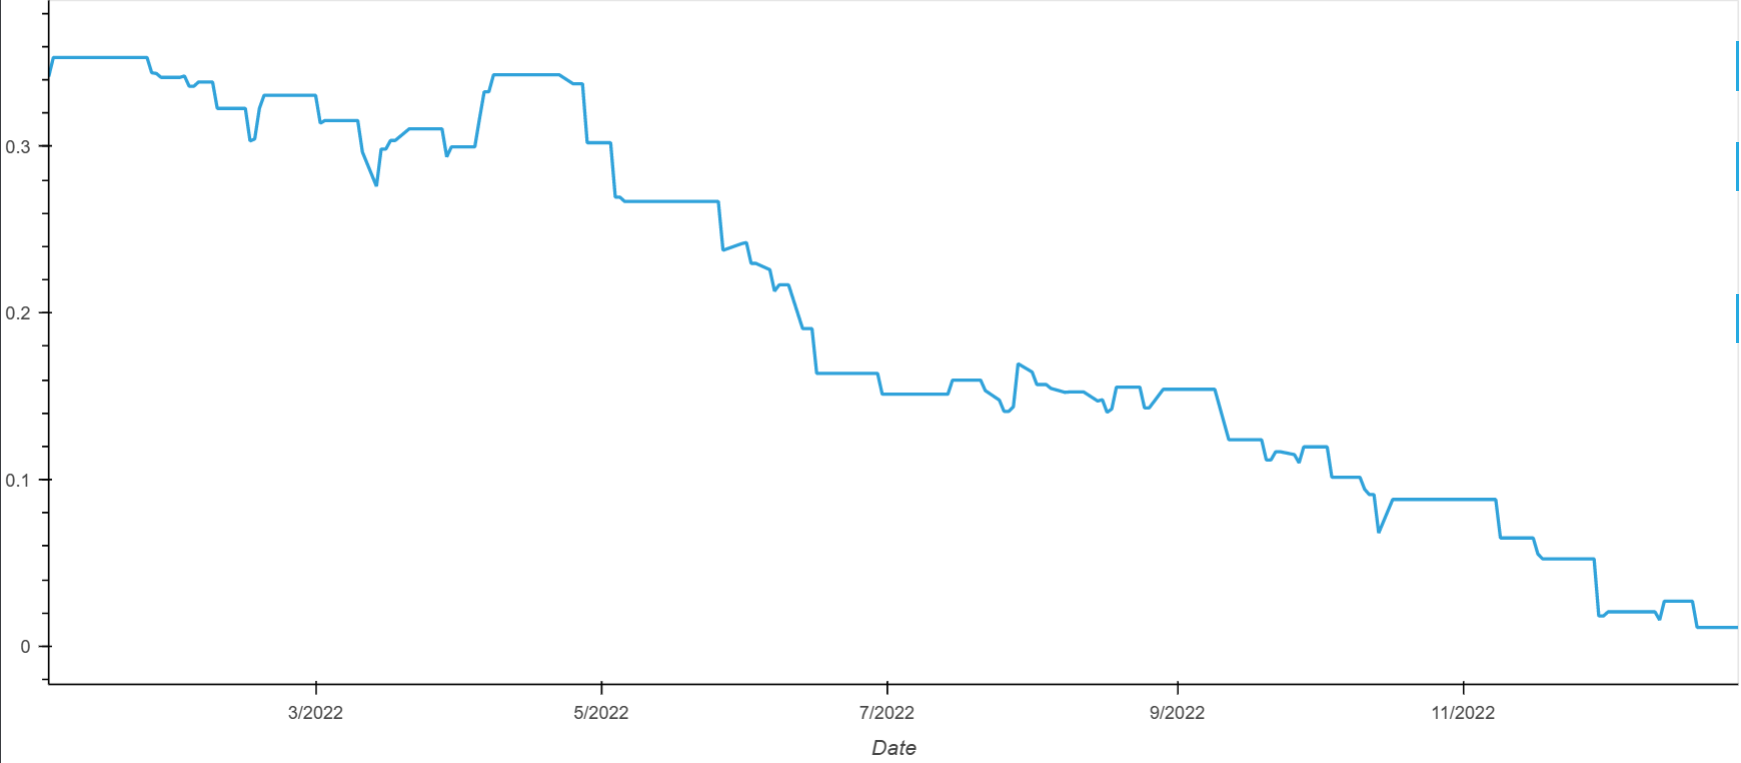
\includegraphics[width=0.8\textwidth]{Images/apple_williams_lma__2.png}
\caption{Cumulative for AAPL (Lookback Period = 14 Days, Breakout Percent = 20, Williams \% R + LMASMA Strategy, Year = 2022)}
\label{fig:entryexit1}
\end{figure}